
\documentclass[12pt]{standalone}
\usepackage{amssymb,latexsym, amsmath,graphics}
\usepackage{amsthm}
\usepackage{setspace}

\doublespacing

\usepackage{pgf}
\usepackage{tikz}
\usetikzlibrary{arrows,automata}
\usetikzlibrary{positioning}



\begin{document}
\pagestyle{empty}
 \centering
 % Main layout borrowed from 
 % Gray Code in 4-cube
% Author: Yury Chebiryak <http://yury.chebiryak.name/index.html>
%\documentclass{article}
%\usepackage{tikz}

 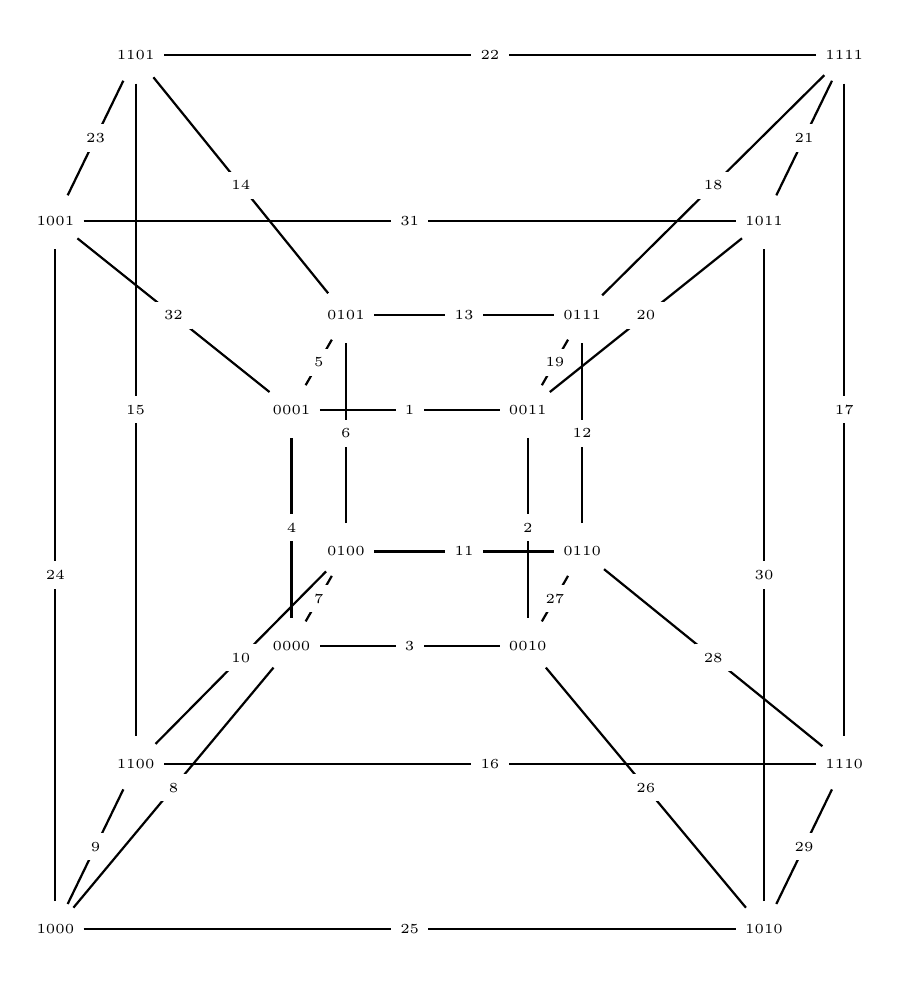
\begin{tikzpicture} [scale=3]
	 \tikzstyle{vertex}=[circle,minimum size=20pt,inner sep=0pt]
	 \tikzstyle{edge} = [draw,thick,-,black]
%	 \node[vertex] (v0) at (0,0) {$0000$};
%	 \node[vertex] (v1) at (0,1) {$0001$};
%	 \node[vertex] (v2) at (1,0) {$0010$};
%	 \node[vertex] (v3) at (1,1) {$0011$};
%	 \node[vertex] (v4) at (0.23, 0.4) {$0100$};
%	 \node[vertex] (v5) at (0.23,1.4) {$0101$};
%	 \node[vertex] (v6) at (1.23,0.4) {$0110$};
%	 \node[vertex] (v7) at (1.23,1.4) {$0111$};
	 \node[vertex] (v0) at (0,.2) {{\tiny $0000$}};
	 \node[vertex] (v1) at (0,1.2) {{\tiny $0001$}};
	 \node[vertex] (v2) at (1,0.2) {{\tiny $0010$}};
	 \node[vertex] (v3) at (1,1.2) {{\tiny $0011$}};
	 \node[vertex] (v4) at (0.23, 0.6) {{\tiny $0100$}};
	 \node[vertex] (v5) at (0.23,1.6) {{\tiny $0101$}};
	 \node[vertex] (v6) at (1.23,0.6) {{\tiny $0110$}};
	 \node[vertex] (v7) at (1.23,1.6) {{\tiny $0111$}};
	 
	 \node[vertex] (v8) at (-1,-1) {{\tiny $1000$}};
	 \node[vertex] (v9) at (-1,2) {{\tiny $1001$}};
	 \node[vertex] (v13) at (-0.66,2.7) {{\tiny $1101$}};
	 \node[vertex] (v12) at (-0.66,-0.3) {{\tiny $1100$}};
	 \node[vertex] (v10) at (2,-1) {{\tiny $1010$}};
	 \node[vertex] (v14) at (2.34,-0.3) {{\tiny $1110$}};
	 \node[vertex] (v11) at (2,2) {{\tiny $1011$}};
	 \node[vertex] (v15) at (2.34,2.7) {{\tiny $1111$}};
	 
	 \draw[edge] (v1) -- (v3) node[midway, fill=white]{{\tiny 1}};
	 \draw[edge] (v3) -- (v2) node[midway, fill=white]{{\tiny 2}};
	 \draw[edge] (v2) -- (v0) node[midway, fill=white]{{\tiny 3}};
	 \draw[edge] (v0) -- (v1) node[midway, fill=white]{{\tiny 4}};
	 
	 \draw[edge] (v0) -- (v4) node[midway, fill=white]{{\tiny 7}};
	 \draw[edge] (v4) -- (v5) node[midway, fill=white]{{\tiny 6}};
	 \draw[edge] (v5) -- (v1) node[midway, fill=white]{{\tiny 5}};
	 
	 \draw[edge] (v2) -- (v6) node[midway, fill=white]{{\tiny 27}};
	 \draw[edge] (v6) -- (v7) node[midway, fill=white]{{\tiny 12}};
	 \draw[edge] (v7) -- (v3) node[midway, fill=white]{{\tiny 19}};
	 \draw[edge] (v4) -- (v6) node[midway, fill=white]{{\tiny 11}};
	 \draw[edge] (v7) -- (v5) node[midway, fill=white]{{\tiny 13}};
	 
	 \draw[edge] (v8) -- (v9) node[midway, fill=white]{{\tiny 24}};
	 \draw[edge] (v9) -- (v13) node[midway, fill=white]{{\tiny 23}};
	 \draw[edge] (v13) -- (v12) node[midway, fill=white]{{\tiny 15}};
	 \draw[edge] (v4) -- (v12) node[midway, fill=white]{{\tiny 10}};
	 \draw[edge] (v12) -- (v8) node[midway, fill=white]{{\tiny 9}};
	 \draw[edge] (v8) -- (v0) node[midway, fill=white]{{\tiny 8}};
	 \draw[edge] (v1) -- (v9) node[midway, fill=white]{{\tiny 32}};
	 \draw[edge] (v13) -- (v5) node[midway, fill=white]{{\tiny 14}};
	 \draw[edge] (v2) -- (v10) node[midway, fill=white]{{\tiny 26}};
	 \draw[edge] (v10) -- (v14) node[midway, fill=white]{{\tiny 29}};
	 \draw[edge] (v14) -- (v6) node[midway, fill=white]{{\tiny 28}};
	 \draw[edge] (v8) -- (v10) node[midway, fill=white]{{\tiny 25}};
	 \draw[edge] (v14) -- (v12) node[midway, fill=white]{{\tiny 16}};
	 \draw[edge] (v3) -- (v11) node[midway, fill=white]{{\tiny 20}};
	 \draw[edge] (v11) -- (v15) node[midway, fill=white]{{\tiny 21}};
	 \draw[edge] (v15) -- (v7) node[midway, fill=white]{{\tiny 18}};
	 \draw[edge] (v10) -- (v11) node[midway, fill=white]{{\tiny 30}};
	 \draw[edge] (v15) -- (v14) node[midway, fill=white]{{\tiny 17}};
	 \draw[edge] (v9) -- (v11) node[midway, fill=white]{{\tiny 31}};
	 \draw[edge] (v15) -- (v13) node[midway, fill=white]{{\tiny 22}};
	% \node[] at (.66,-1.25) {\Huge $Q_4$};
 \end{tikzpicture}
\end{document}